% !TEX root = ../report.tex
\section{User Experience}

\subsection{Sender User Experience}

\begin{figure}[H]
 \makebox[\textwidth][c]{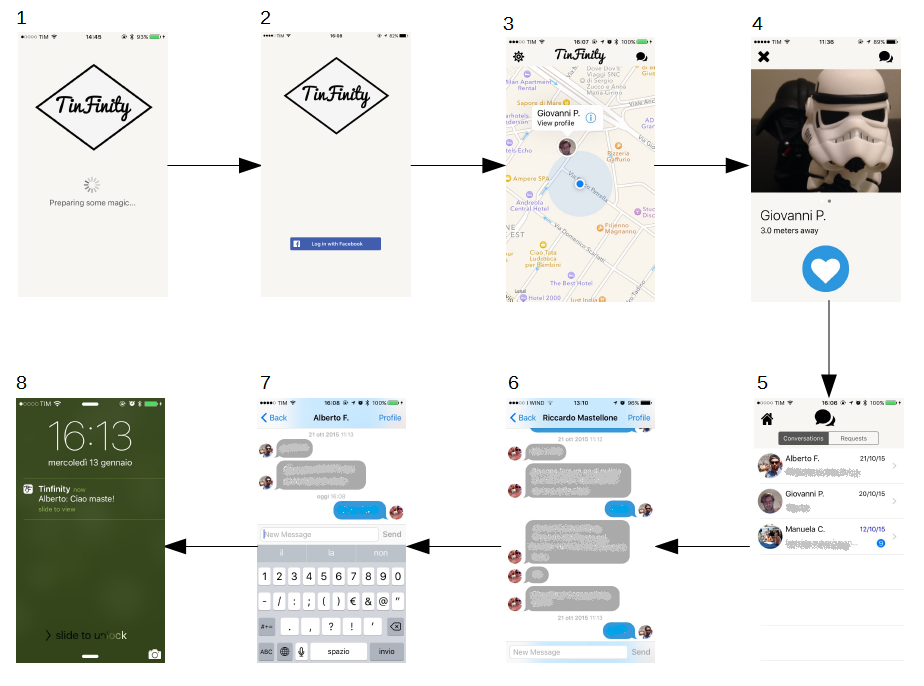
\includegraphics[width=1.6\textwidth]{./images/ux_sender.png}}%
\caption{Sender User Experience}
\end{figure}

\begin{enumerate}
\item The application launcher contacts the server in order to retrieve to check if there isa already a valid login token present

\item From the login view the user can inserts his Facebook username and password and log in to the application

\item From the main view the user can see the people around him and choose to look at an interesting profile

\item The user can send a frienship request

\item[5--8] When and if the other user accept the friendship request, they can start chatting as a normal chat application.
\end{enumerate}


\subsection{Receiver User Experience}

\begin{figure}[H]
 \makebox[\textwidth][c]{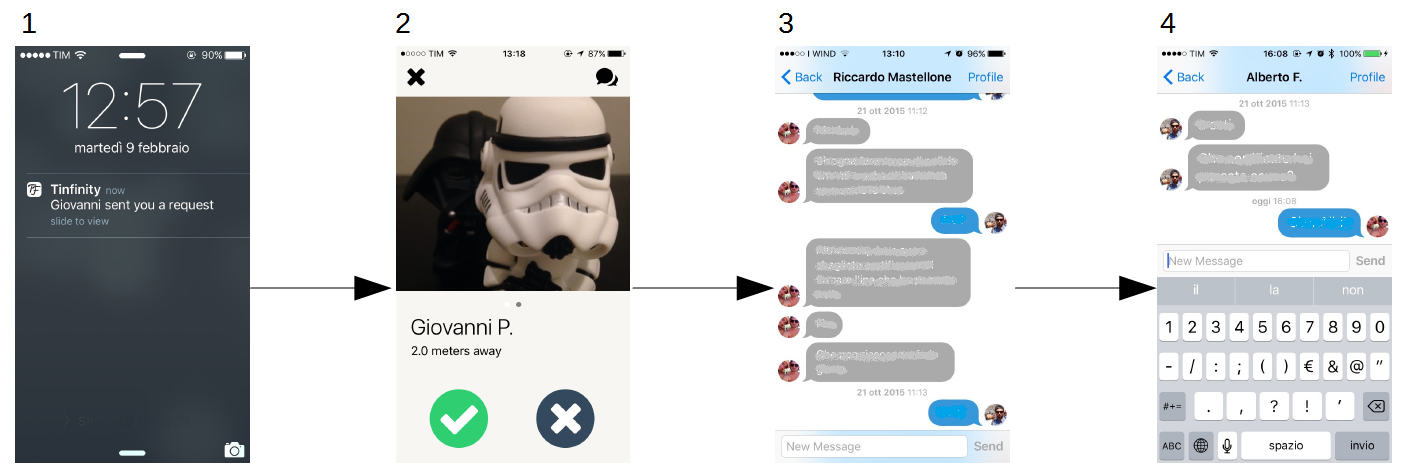
\includegraphics[width=1.6\textwidth]{./images/ux_receiver.png}}%
\caption{Receiver User Experience}
\end{figure}

\begin{enumerate}
\item The user receive a notification about a received friendhip request 

\item The user can choose if the request has to be accepted or declined


\item[3--4] If the friendship is granted they can start chatting as a normal chat application.
\end{enumerate}

\newpage

\subsection{Photo selection User Experience}

\begin{figure}[H]
 \makebox[\textwidth][c]{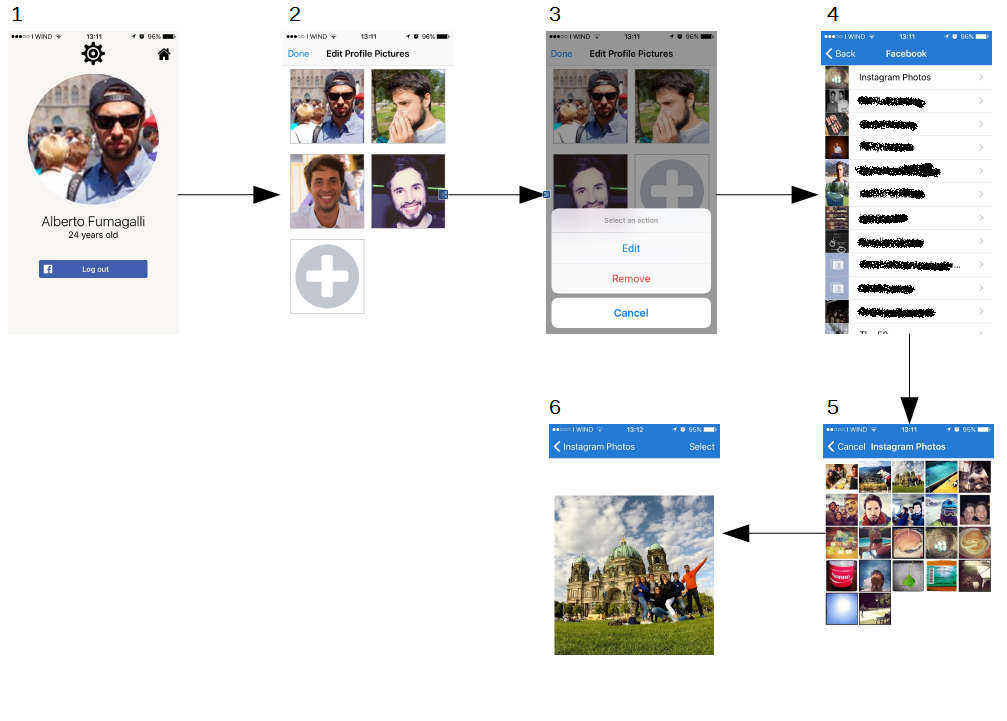
\includegraphics[width=1.6\textwidth]{./images/ux_photo_change.png}}%
\caption{Photo selection User Experience}
\end{figure}

\begin{enumerate}
\item From the settings view the user can tap on his photo profile in order to modify it or add other photos which will be visible by other users.

\item The user can tap on the '+' button and chose whether to add or change a current photo

\item All the photo albums of the Facebook account are displayed 

\item  All the photos of the selected album are displayed

\item  Finally tap on the select button the displayed photo is added to the user profile

\end{enumerate}